\newpage
\section{Generalised Negative Binomial Distribution}
\subsection*{Introduction}
The \emph{negative binomial} distribution, NB, was first proposed almost 
100 years ago in 1920 by Greenwood \& Woods, \cite{greenwood1920inquiry}, 
but its generalisation for both \emph{binomial} and NB distributions called the 
\emph{generalised negative binomial distribution}, GNB, was discovered 
more then 50 years later by Jain \& Consul (1971), \cite{jain1971generalized}. 
The PMF of the GNB is defined for $0<\alpha<1$ and $|\alpha \beta| < 1$ 
and reads in Jain \& Consul paper
\begin{align*}
b_{\beta}(x,n,\alpha) &= 
\frac{n \; \Gamma(n+\beta x)}{x! \;\Gamma(n + \beta x - x +1)}  \; \alpha^x (1-\alpha)^{n+\beta x-x}, n>0, x=0,1,2,3,...
\end{align*}
such that $b_{\beta}(x,n,\alpha) = 0 \text{ for } x \leq m \text{ if } n+\beta m < 0.$\\
Interestingly, following distributions are special cases of the GNB distribution
\begin{itemize}
\item 
binomial, B(n,p)
\item 
negative binomial, NB(r,p)\footnote{This corresponds to the NB1 parameterisation 
of the negative binomial distribution in ProbOnto, \cite{Swat:2015a}.}
\item 
inverse binomial, IB(k,p)
\end{itemize}
which will be shown in the following sections. 

\begin{figure}[ht!]
\centering
  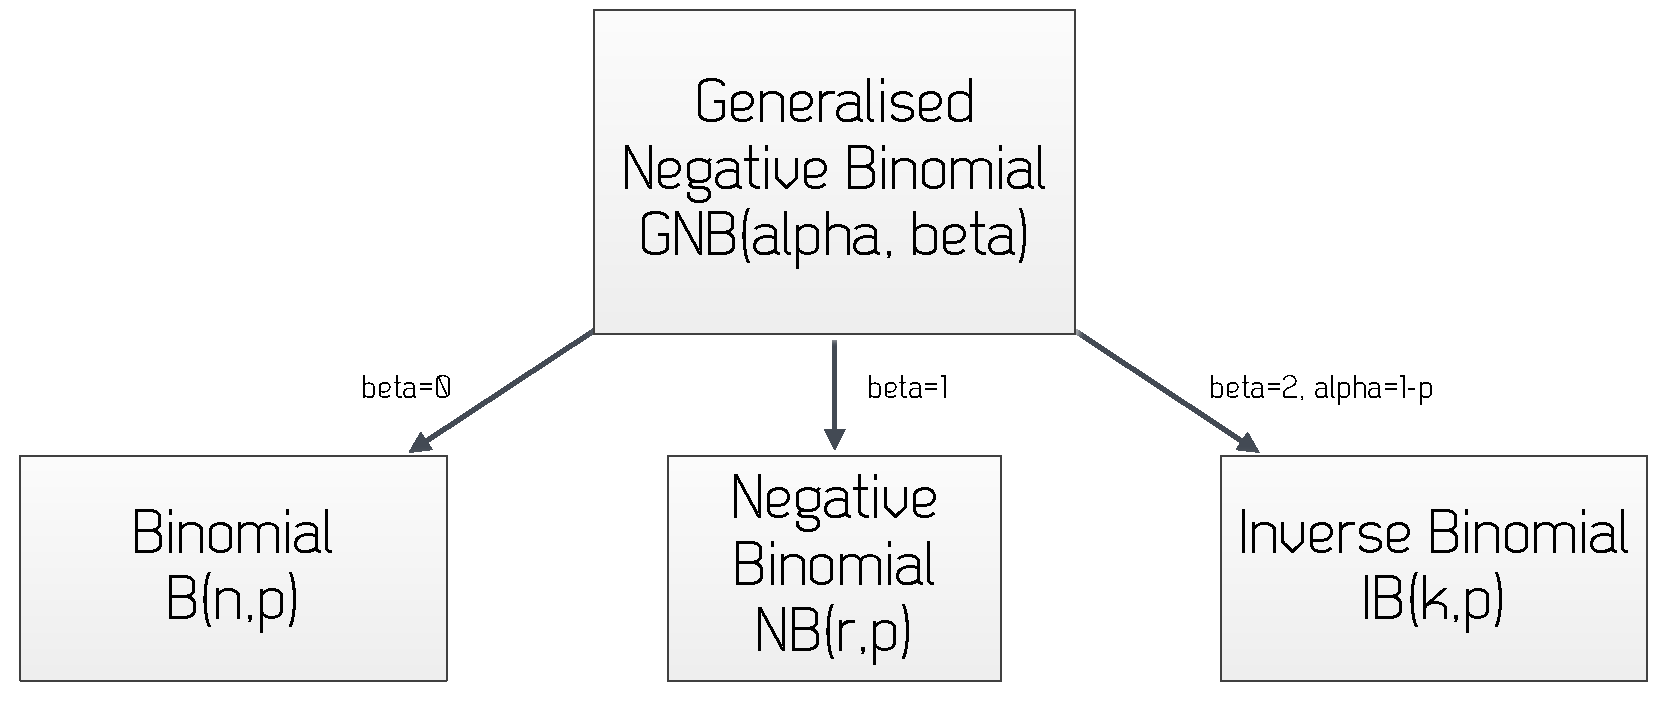
\includegraphics[width=120mm]{pics/GNBspecialCases.pdf}
 \caption{GNB and its family.}
 \label{fig:GNBspecialCases}
\end{figure}


\subsection*{GNB($\alpha$,$\beta$) $\rightarrow$ B($n$,$p$)}
According to Jain \& Consul, \cite{jain1971generalized}, GNB reduces to B for $\beta = 0$ and 
indeed this can be shown (replacing $\alpha$ with $p$) as follows
\begin{align*}
 b_{\beta}(x,n,\alpha) \rightarrow P_{B}(x;n,p): %= \binom {k+r-1}k (1-p)^r p^k \nonumber
 \frac{n \; \Gamma(n+\beta x)}{x! \;\Gamma(n + \beta x - x +1)}  \; \alpha^x (1-\alpha)^{n+\beta x-x} \rightarrow 
\frac{n \; \Gamma(n)}{x! \;\Gamma(n - x +1)}  \; p^x (1-p	)^{n-x} 
\end{align*}
with the first term in the last expression $\frac{n \; \Gamma(n)}{x! \;\Gamma(n - x +1)} = \frac{n (n-1)!}{x! (n-x)!} 
= \frac{n!}{x!(n-x)!} = {n \choose x}$ we get the expected result
\begin{align*}
P_{B}(x;n,p) = {n \choose x} p^x (1-p)^{n-x}. % \quad \text{ with } \quad 0<p<1, n>0, x=0,1,2,3,....
\end{align*}

\subsection*{GNB($\alpha$,$\beta$) $\rightarrow$ NB($r$,$p$)}
According also to Jain \& Consul, \cite{jain1971generalized}, GNB reduces to NB for $\beta = 1$ and 
indeed this can be shown (replacing $\alpha$ with $p$ and $n$ with $r$) as follows
\begin{align*}
 b_{\beta}(x,n,\alpha) \rightarrow P_{N\!B}(x;r,p):
 \frac{n \; \Gamma(n+\beta x)}{x! \;\Gamma(n + \beta x - x +1)}  \; \alpha^x (1-\alpha)^{n+\beta x-x} \rightarrow 
\frac{r \; \Gamma(r + x)}{x! \;\Gamma(r + 1)}  \; p^x (1-p)^{r} 
\end{align*}
with the first term $\frac{r \; \Gamma(r + x)}{x! \;\Gamma(r + 1)} = \frac{r \; (r + x - 1)!}{x! \;r!} = \frac{(r + x - 1)!}{x! \;(r-1)!}
= {r + x - 1 \choose x}$ we get the correct PMF
\begin{align*}
P_{N\!B}(x;r,p) = {r + x - 1 \choose x} p^x (1-p)^r  .
\end{align*}


\subsection*{GNB($\alpha$,$\beta$) $\rightarrow$ IB($k$,$p$)}
Yanagimoto, \cite{yanagimoto1989inverse}, proposed the \emph{inverse binomial} 
distribution as another special case of GNB for $\beta = 2, \alpha=1-p$ and $n=k$, which 
can be derived as the following shows 
\begin{align*}
b_{\beta}(x,n,\alpha) \rightarrow P_{I\!B}(x;k,p):
 \frac{n \; \Gamma(n+\beta x)}{x! \;\Gamma(n + \beta x - x +1)}  \; \alpha^x (1-\alpha)^{n+\beta x-x} \rightarrow 
\frac{k \; \Gamma(k + 2x)}{x! \;\Gamma(k + x + 1)}  \; (1-p)^x p^{k+x} 
\end{align*}
and the result follows in agreement with the formulation in \cite{yanagimoto1989inverse}, i.e.
\begin{align*}
P_{I\!B}(x;k,p) = \frac{k \; \Gamma(2x + k)}{\Gamma(x+1) \;\Gamma(x + k + 1)}  \; p^{k+x} (1-p)^x ,
\end{align*}
and from $|\alpha \beta| < 1$ and $0<\alpha<1$ one can derive the required condition for p, $1/2 < p < 1$.\\
Interestingly, IB has a medical application. Yanagimoto, \cite{yanagimoto1989inverse}, 
used the distribution it estimate the proportion of discharged patients who can be 
expected to stay completely free from some disease. In the original paper a dataset
for relapse of pulmonary tuberculosis was analysed.

%\section*{Appplications}
%\begin{itemize}
%\item 
%Binomial
%\begin{itemize}
%\item 
%\end{itemize}
%\item 
%Negative Binomial
%\begin{itemize}
%\item 
%\end{itemize}
%\item 
%Inverse Binomial
%\begin{itemize}
%\item 
%\end{itemize}
%\end{itemize}


\section*{Bios}
Here short bios of the people behind these distributions:

\begin{itemize}
\item 
Greenwood and Yule (1920), 'An inquiry into the nature of frequency 
distributions representative of multiple happenings with particular 
reference to the occurrence of multiple attacks of disease or of 
repeated accidents':
\begin{itemize}
\item 
Major Greenwood FRS (9 August 1880 - 5 October 1949) was 
an English epidemiologist and statistician born in Shoreditch in 
London's East End. He was elected President of the Royal Statistical 
Society in 1934 and awarded its Guy Medal in Gold in 1945.
\item 
Udny Yule FRS (18 February 1871 - 26 June 1951) was a 
Scottish statistician, born in Morham, near Haddington. He was active 
in the Royal Statistical Society, was also awarded its Guy Medal in Gold 
in 1911, and served as its president in 1924-26.
\end{itemize}
\item 
Jain and Consul (1971), 'A generalized negative binomial distribution':
\begin{itemize}
\item 
about Jain nothing is known on the web.
\item 
Prem C. Consul is professor emeritus at the Department 
of Mathematics and Statistics, University of Calgary, and author of 
books on Generalised Poisson and Lagrangian distributions 
\url{http://math.ucalgary.ca/math_unitis/profiles/prem-c-consul}
\end{itemize}
\item 
Yanagimoto (1989), 'The inverse binomial distribution as a statistical 
model':
\begin{itemize}
\item 
Takemi Yanagimoto - professor at the Institute of 
Statistical Mathematics in Tokyo.
\url{http://www.ism.ac.jp/~yanagmt/eng.html}
\end{itemize}
\end{itemize}

\newpage
\section{Parameterisations of NB1}
\label{app:sec:NB1discussion}

There are essentially three ways to formulate and interpret an experiment for 
the independent Bernoulli trials with a fixed number of outcomes (successes or
failures). The NB model which formalises this experiment is formulated using two 
out of three following parameters dependent on the formulation: 
number of trials (i.e. total number successes or failures), number of successes, 
number of failures. 

Below we list the formulations of the experimental goal: the estimation of the 
probability distribution in a series of Bernoulli trials for
\begin{itemize}
\item 
observing k failures before obtaining the r$^{th}$ success (most common)
\item 
obtaining r successes until r$^{th}$ failures have occurred
\item 
number of trials, $n$, required to before the r$^{th}$ success occurs 
\end{itemize}
The first one is most common with the last two options encountered
only in very few cases.

The UncertML, based on the english version of Wikipedia, uses the second 
interpretation of this distribution. In the current version of ProbOnto we have 
reformulated it to align with the vast majority of sources. 
Otherwise, mistake are likely as the target tools e.g. Matlab, R and 
winBUGS, to mention here only few, use the most common form.

See Table \ref{figTable:NB1forms} below for the overview with references of the used definitions and 
the implementations of NB in target tools and references.


\subsection*{English Wikipedia}
\textbf{Interpretation}: distribution of the number of successes, \emph{k}, until \emph{r} failures have occurred.
\begin{align*}
P_{N\!B}(k;r,p) = {k + r - 1 \choose k} p^k (1-p)^r, \quad \operatorname E(X\!=\!k)=\frac{rp}{(1-p)}
\end{align*}
\begin{itemize}
\item 
Support
\begin{itemize}
\item 
$k \in \{ 0, 1, 2, 3, \dots\}$ -- number of \textbf{successes}
\end{itemize}
\item 
Parameters 
\begin{itemize}
\item 
$r > 0$ -- number of \textbf{failures} until the experiment is stopped
\item 
$p \in (0,1)$ -- success probability in each experiment
\end{itemize}
\end{itemize}


\subsection*{French Wikipedia}
\textbf{Interpretation}: distribution of the number of failures, \emph{k}, before obtaining \emph{n} successes
\begin{align*}
P_{N\!B}(k;n,p) = {k + n - 1 \choose k} p^n (1-p)^k, \quad \operatorname E(X\!=\!k)=\frac{n(1-p)}{p}
\end{align*}
% This experiment continues until a given number n of success. The random variable representing the number of failures (before obtaining the given number n of success) then follows a negative binomial distribution. Its parameters are n, the number of expected success, and p, the probability of success.
\begin{itemize}
\item 
Support
\begin{itemize}
\item 
$k \in \{ 0, 1, 2, 3, \dots\}$ -- number of \textbf{failures}
\end{itemize}
\item 
Parameters 
\begin{itemize}
\item 
$n > 0$ -- number of \textbf{successes} until the experiment is stopped (fr: \emph{le nombre de succ\`es attendus})
\item 
$p \in (0,1)$ -- success probability in each experiment (fr: \emph{la probabilit\`e d'un succ\`es})
\end{itemize}
\end{itemize}

\subsection*{German Wikipedia}
The german Wiki page describes two alternative representations and interpolations
of this distribution. We present here there one which is presented in the overview 
box on the right-hand side, denoted as the alternative representation.\\
\textbf{Interpretation}: distribution of the number of failures, \emph{k}, before obtaining \emph{r} successes. 
(ger.: \emph{NB Distribution beschreibt die Anzahl, k, der Misserfolge bis zum Eintreten des r-ten Erfolgs.})
\begin{align*}
P_{N\!B}(k;r,p) = {k + r - 1 \choose k} p^r (1-p)^k, \quad \operatorname E(X\!=\!k)=\frac{r(1-p)}{p}
\end{align*}
\begin{itemize}
\item 
Support
\begin{itemize}
\item 
$k \in \{ 0, 1, 2, 3, \dots\}$ -- number of \textbf{failures} (ger: \emph{Anzahl Misserfolge})
\end{itemize}
\item 
Parameters 
\begin{itemize}
\item 
$r > 0$ -- number of \textbf{successes} until the experiment is stopped (ger: \emph{Anzahl Erfolge bis zum Abbruch})
\item 
$p \in (0,1)$ -- success probability in each experiment, (ger: \emph{Einzel-Erfolgs-Wahrscheinlichkeit})
\end{itemize}
\end{itemize}
\begin{align*}
P_{N\!B}(k;r,p) = {k + r - 1 \choose k} p^r (1-p)^k  .
\end{align*}

All the Wikipedia article were accessed on 4th August 2015.

\subsection{Implementation in software tools and reference sources}
\label{subsec:NB1implementations}

\captionsetup[longtable]{skip=1em}
\LTcapwidth=.95\textwidth
\begin{center}
\setlength{\tabcolsep}{7pt}
%\small
\renewcommand{\arraystretch}{1.1}%
\begin{longtable}{lcccc}
  \hline
  \hline
  %header
  Source 		& PMF	& Parameter 	& Support & Support variable \\ [-0.5ex]
  			&		&			&		& interpretation \\
  \hline
  \hline
  \multicolumn{5}{c}{\textit{Type 1}}  \\
  \multicolumn{5}{c}{\textit{probability of observing a fixed number of failures before certain number of success}}  \\
  \hline
  \hline
   \Gape[.4cm][0cm]{}Hilbe (2007), \cite{hilbe2011negative}	& ${y+r-1 \choose y} p^r (1-p)^\textbf{y} $ & $0 < p < 1$ & $0 \leq y < \infty$ & number of failures\\[0.5ex]
  \hline
  \Gape[.4cm][0cm]{}Forbes et al. (2011), \cite{forbes2011statistical} 	& ${x+r-1 \choose x} p^r (1-p)^\textbf{x} $ & $0 < p < 1$ & $0 \leq x < \infty$ & number of failures\\[0.5ex]
  \hline
  \Gape[.4cm][0cm]{}Leemis (2008), \cite{Leemis:2008tg}		& ${x+r-1 \choose x} p^r (1-p)^\textbf{x}$ & $0 < p < 1$ & $0 \leq x < \infty$ & --\\[0.5ex]
  \hline
  \Gape[.4cm][0cm]{}R -- \emph{stats} package & $\frac{\Gamma(x+n)}{\Gamma(n)  x!} p^n (1-p)^\textbf{x}$ & $0 < p \leq 1$ & $x \in 0,1,...$ & number of failures \\[0.5ex]
  \hline
  \Gape[.4cm][0cm]{}Matlab -- Stats Toolbox 	& ${x+r-1 \choose x} p^r (1-p)^\textbf{x}$ & $0 < p < 1$ & $0 \leq x < \infty$ & number of failures \\[0.5ex]
  \hline
  \Gape[.4cm][0cm]{}Devroye (1986),\cite{Devroye:1986nx}	& ${x+n-1 \choose x} p^n (1-p)^\textbf{x}$ & $p \in (0,1)$ & $x \geq 0$ & number of failures \\[0.5ex]
  \hline
  \Gape[.4cm][0cm]{}Dobson (2002) 			& ${y+r-1 \choose y} p^r (1-p)^\textbf{y}$ & -- & -- & --\\[0.5ex]
  \hline
  \Gape[.4cm][0cm]{}VGAM 			& ${y+k-1 \choose y} p^k (1-p)^\textbf{y}$ & $0 < p < 1$ & $x \in 0,1,2,...$ & -- \\[0.5ex]
  \hline
  \Gape[.4cm][0cm]{}winBUGS 			& ${x+r-1 \choose x} p^r (1-p)^\textbf{x}$ & -- & $0 \leq x < \infty$ & -- \\[0.5ex]
  \hline
  \Gape[.4cm][0cm]{}UUPDE 			& ${m+n-1 \choose n-1} p^n (1-p)^\textbf{m}$ & $0 < p \leq 1$ & $m \in 0,1,2,...$ & -- \\[0.5ex]
  \hline
  \Gape[.4cm][0cm]{}VoseSoftware 		& ${s+x-1 \choose x} p^s (1-p)^\textbf{x}$ & $0 < p \leq 1$ & $x \in 0,1,...$ & number of failures \\[0.5ex]
  \hline
  \Gape[.4cm][0cm]{}boost.org 			& ${x+r-1 \choose x} p^r (1-p)^\textbf{x}$ & -- & -- & number of failures \\[0.5ex]
  \hline
  \Gape[.4cm][0cm]{}Mathwave 		& ${x+n-1 \choose x} p^n (1-p)^\textbf{x}$ & $0 < p < 1$ & $x \in 0,1,...$ & -- \\[0.5ex]
  \hline
  \Gape[.4cm][0cm]{}Wolfram 			& ${x+r-1 \choose x} p^r (1-p)^\textbf{x}$ & -- & -- & number of failures \\[0.5ex]
  \hline
  \Gape[.4cm][0cm]{}French Wikipedia 	& ${k+r-1 \choose k} p^r (1-p)^\textbf{k}$ & $p \in (0,1)$ & $k \in 0,1,2,3,...$& number of failures \\[0.5ex]
  \hline
  \Gape[.4cm][0cm]{}German Wikipedia 	& ${k+r-1 \choose k} p^r (1-p)^\textbf{k}$ & $p \in (0,1)$ & $k \in 0,1,2,3,...$ & number of failures \\[0.5ex]
  \hline
  \hline
  \multicolumn{5}{c}{\textit{Type 2}}	\\
  \multicolumn{5}{c}{\textit{probability of observing a fixed number of successes before certain number of failures}}	\\
  \hline
  \Gape[.4cm][0cm]{}Agresti (2013),\cite{Agresti:2013pd} 		& ${y+k-1 \choose y} (1-p)^k p^\textbf{y}$ & -- & $y \in 0,1,2,...$ & number of successes \\[0.5ex]
  \hline
  \Gape[.4cm][0cm]{}English Wikipedia 	& ${k+r-1 \choose k} (1-p)^r p^\textbf{k}$ & $p \in (0,1)$ & $k \in 0,1,2,3,...$ & number of successes \\[0.5ex]
  \hline
  \hline
  \multicolumn{5}{c}{\textit{Type 3}}	\\
  \multicolumn{5}{c}{\textit{probability of number of trials required to achieve certain number of success}}	\\
  \hline
  \Gape[.4cm][0cm]{}Distributome 		& ${x-1 \choose k-1} p^k (1-p)^{\textbf{x}-k}$ & -- & $x \in k,k+1,...$ & number of trials \\[0.5ex]
  \hline
  \Gape[.4cm][0cm]{}Song, Chen (2011)	& ${x-1 \choose k-1} p^k (1-p)^{\textbf{x}-k}$ & $0 \leq p \leq 1$ & $x \in k,k+1,...$ & -- \\[0.5ex]
   \hline 
  \Gape[.4cm][0cm]{}massmatics.de		& ${n-1 \choose r-1} p^r (1-p)^{\textbf{n}-r}$ & $0 \leq p \leq 1$ & $n \in N, n \geq r$ & number of trials \\[0.5ex]
   \hline 
\caption{NB formulation overview}
\label{figTable:NB1forms}
\vspace{-2.5em}
\end{longtable}
\end{center}




















